\begin{figure*}[t]
\centering
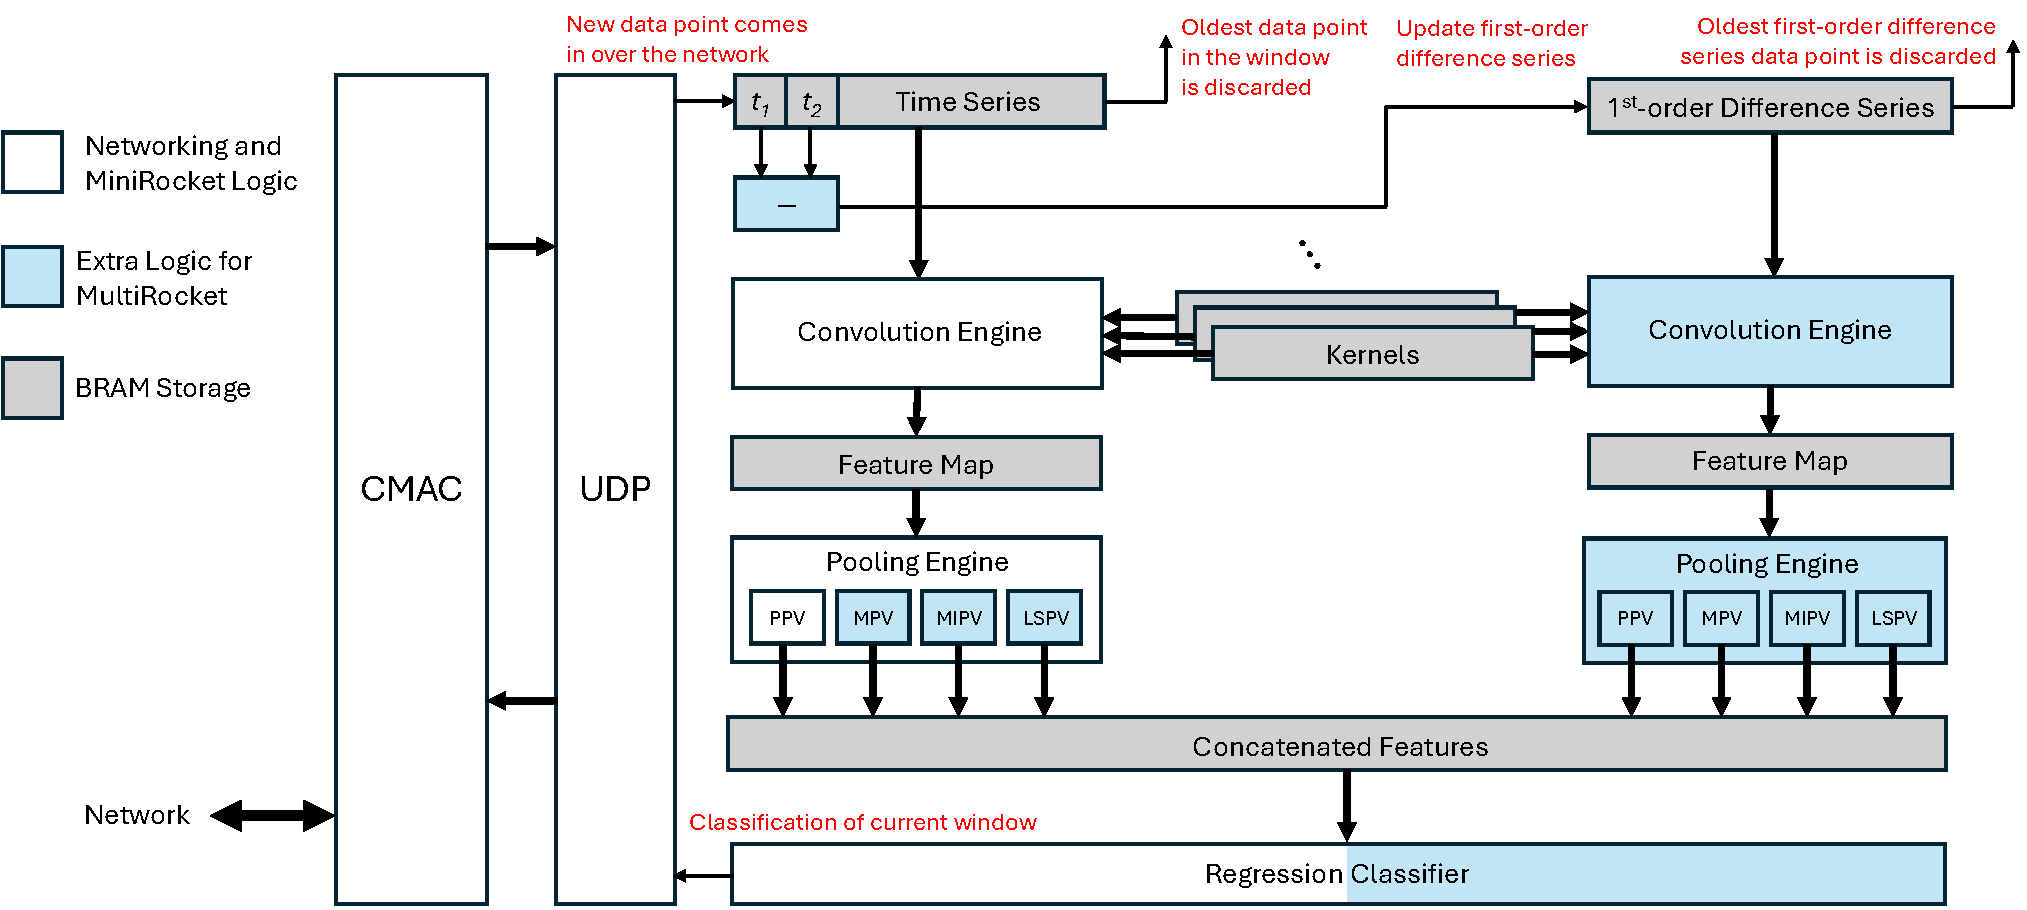
\includegraphics[width=1\linewidth]{Figures/Mini-MultiRocket_Arch.pdf}
\caption{FPGA accelerator for MiniRocket and MultiRocket. A lower-cost MiniRocket-exclusive accelerator can be obtained by removing the logic components shaded blue and any BRAM storage resources read or written exclusively by those components.}
\label{fig:MiniMultiRocket_arch}
\end{figure*}

\section{FPGA Accelerator Architectures}
\label{sec:accelerators}

We present two FPGA accelerator architectures, one for MiniRocket and MultiRocket (Fig. \ref{fig:MiniMultiRocket_arch}), and the other for Hydra (Fig. \ref{fig:Hydra_arch})\footnote{
We did not design an accelerator for Rocket because of the inefficiencies which result from variable-length kernels: either an indexing table would be needed to identify the memory address of each kernel; or the kernels would need to be padded with zeroes so that all kernels have length $11$.}. 
Figs. \ref{fig:MiniMultiRocket_arch} and \ref{fig:Hydra_arch} share a common interface. The time series being classified is streamed over the network; each data-point is a 32-bit float. The \textbf{CMAC} is a 100 Gbps Ethernet port and the \textbf{UDP} block implements the User Datagram Protocol; our testbed does not necessitate reliable transport. The accelerator can also read the time series from DDR or High-Bandwidth Memory (HBM) (not shown).

Time series datapoints arrive one-at-a-time over the network. The accelerator maintains two circular buffers to store the most recent window of sampled datapoints of time series $T$, along with $T$'s first-order difference series $T'$. When a new datapoint arrives, the oldest datapoints in $T$ and $T'$ are discarded and $T'$ is updated by taking the difference between the two most recently sampled datapoints $t_2 - t_1$.

For both accelerators, the total amount of storage required for the two time series, kernels, feature maps, concatenated features, and regression classifier weights fit within the aggregate BRAM capacity of our target FPGA, an AMD Alveo u280. As such, BRAM storage is used exclusively, with most of the space allocated to the kernels.

Both accelerators include Convolution Engines, which are functionally identical. The two MultiRocket Convolution Engines (Fig. \ref{fig:MiniMultiRocket_arch}) are sized to the number of kernels and dilations, whereas Hydra's Group Convolution Engines (Fig. \ref{fig:Hydra_arch}) are sized to the number of kernels and dilations within a kernel group, and then replicated (two Convolution Engines per kernel group). MultiRocket's dual Pooling Engines compute the PPV, MPV, MIPV, and LSPV features, whereas Hydra's Group Pooling Engines compute the minimum hard count and maximum soft count histograms for each group. The regression classifier computes one dot product per class plus and an $\argmax$. Pooling engine and regression classifier details are omitted to conserve space. 

\subsection{Convolution Engine Design}
\label{sec:conv_engine}

A convolution is a sliding dot product computed over time series $T \in \mathbb{R}^n$ with kernel $\omega \in \mathbb{R}^m$, $m < n$. Let $T_{i..j}$ denote the subsequence $\langle t_i, t_{i+1}, \ldots t_{i+j} \rangle$ of $T$; to account for dilation, let $T^{(d)}_{i..j}$ denote subsequence $\langle t_i, t_{i+d}, \ldots t_{i+jd} \rangle$. In other words, $T *_d \ \omega = \langle T^{(d)}_{1..m} \cdot \omega, T^{(d)}_{2..m+1} \cdot \omega, \ldots T^{(d)}_{n-m+1..m} \cdot \omega \rangle$, is a sequence of dot products between $\omega$ and appropriately dilated subsequences of $T$, as shown in Fig. \ref{fig:convolutions}. The Convolution Engine maximizes efficiency through reuse of dot products. 


In our context, $T$ is a streaming time series in which new datapoints arrive at a fixed sampling rate, subject to network variability. When new datapoint $t_0$ arrives, the oldest datapoint $t_n$ is discarded, and indices are adjusted accordingly, $t_i\rightarrow t_{i+1}, 0 \leq i \leq n-1$. Both $T$ and the feature map $T * \Omega$ computed by the Convolution Engine are circular buffers. 

For the purpose of analysis, we extend $T$ to include $t_0$ and perform no index adjustment. The Convolution Engine first computes $T_{1..n} *_d\ \omega$ followed by $T_{0..n-1} *_d\ \omega$ once $t_0$ arrives. We observe that $T_{1..n-1} *_d\ \omega$, a sequence of $n-1$ dot products, is a common subsequence of both $T_{1..n} *_d\ \omega$ and $T_{0..n-1} *_d\ \omega$. To compute $T_{0..n-1} *_d\ \omega$, the Convolution Engine removes $T^{(d)}_{n -(m+1)d..n}$ from $T_{1..n} *_d\ \omega$ and prepends $T^{(d)}_{0..m-1} \cdot \omega$.

As shown in Fig. \ref{fig:convolution_engine}, the Convolution Engine must also account for padding (i.e., leading/trailing zeros.). Let $0^\alpha \cdot T \cdot 0^\beta$ denote $T$ padded with $\alpha \geq0$ leading zeros and $\beta \geq 0$ trailing zeros. When new datapoints arrive, only $T$ is adjusted: when $t_0$ arrives and $t_n$ is discarded, the padded time series transitions from $0^\alpha \cdot T_{1..n} \cdot 0^\beta$ to $0^\alpha \cdot T_{0..n-1} \cdot 0^\beta$. The Convolution Engine computes feature maps $0^\alpha \cdot  T_{1..n} \cdot 0^\beta *_d \omega$ and $0^\alpha \cdot T_{0..n-1} \cdot 0^\beta *_d \omega$, noting that $T_{1..n-1} *_d\ \omega$ remains common to feature maps, but dot products involving the padding are not. Fig. \ref{fig:convolution_engine} shows an example where $\alpha = 4$ and $\beta = 0$. 

The two convolutions are decomposed as
\begin{equation}
\begin{aligned}
    0^\alpha \cdot T_{1..n} \cdot 0^\beta *_d \omega = &(0^\alpha \cdot T_{1..m-1} *_d\ \omega) \cdot \\
    &(T_{1..n} *_d\ \omega) \cdot \\
    &(T_{m-n+2..n} \cdot 0^\beta *_d\ \omega),
    \label{eq:streaming_conv_padding_1..n}
\end{aligned}
\end{equation}
and
\begin{equation}
\begin{aligned}
    0^\alpha \cdot T_{0..n-1} \cdot 0^\beta *_d \omega = &(0^\alpha \cdot T_{0..m-2} *_d\ \omega) \cdot \\
    &(T_{0..n-1} *_d\ \omega) \cdot \\
    &(T_{m-n+1..n-1} \cdot 0^\beta *_d\ \omega).
    \label{eq:streaming_conv_padding_0..n-1}
\end{aligned}
\end{equation}
Eq. (\ref{eq:streaming_conv_padding_0..n-1}) is then rewritten to reuse $T_{1..n-1} *_d\ \omega$:
\begin{equation}
\begin{aligned}
    0^\alpha \cdot T_{0..n-1} \cdot 0^\beta *_d \omega = &(0^\alpha \cdot T_{0..m-2} *_d\ \omega) \cdot \\
    &\langle T_{0..m-1} \cdot \omega\rangle \cdot (T_{1..n-1} *_d\ \omega) \cdot \\
    &(T_{m-n+1..n-1} \cdot 0^\beta *_d\ \omega).
    \label{eq:streaming_conv_padding_0..n-1_rewrite}
\end{aligned}
\end{equation}

Without reuse, each convolution computes $\alpha + \beta + (n-m) + 1$ dot products, which is reduced to $\alpha + \beta + 1$ with reuse. Aggregated across all kernels and dilations, the number of dot products computed by the Convolution Engine is reduced from $|\Omega||D|(\alpha + \beta + (n-m) + 1)$ to $|\Omega||D|(\alpha + \beta + 1)$. 



%\subsection{MiniRocket and MultiRocket Accelerator}
%\label{sec:MiniMultiRocket_accelerator}

%The accelerator shown in Fig. \ref{fig:MiniMultiRocket_arch} can implement both MiniRocket and MultiRocket, and can be subsetted to implement MiniRocket exclusively at a lower cost. Without loss of generality, we present the full MultiRocket functionality here. 
%Two convolution engines compute feature maps $T\times\Omega$ and $T'\times\Omega$ in parallel. In parallel, two pooling engines compute feature vectors $F_{PPV}(T * \Omega) \cdot F_{MPV}(T * \Omega) \cdot F_{MIPV}(T * \Omega) \cdot F_{LSPV}(T * \Omega)$ and $F_{PPV}(T' * \Omega) \cdot F_{MPV}(T' * \Omega) \cdot F_{MIPV}(T' * \Omega) \cdot F_{LSPV}(T' * \Omega)$, which are then concatenated and sent to the regression classifier. The predicted class is then transmitted back across the network or written to HBM. 




\begin{figure*}[t]
\centering
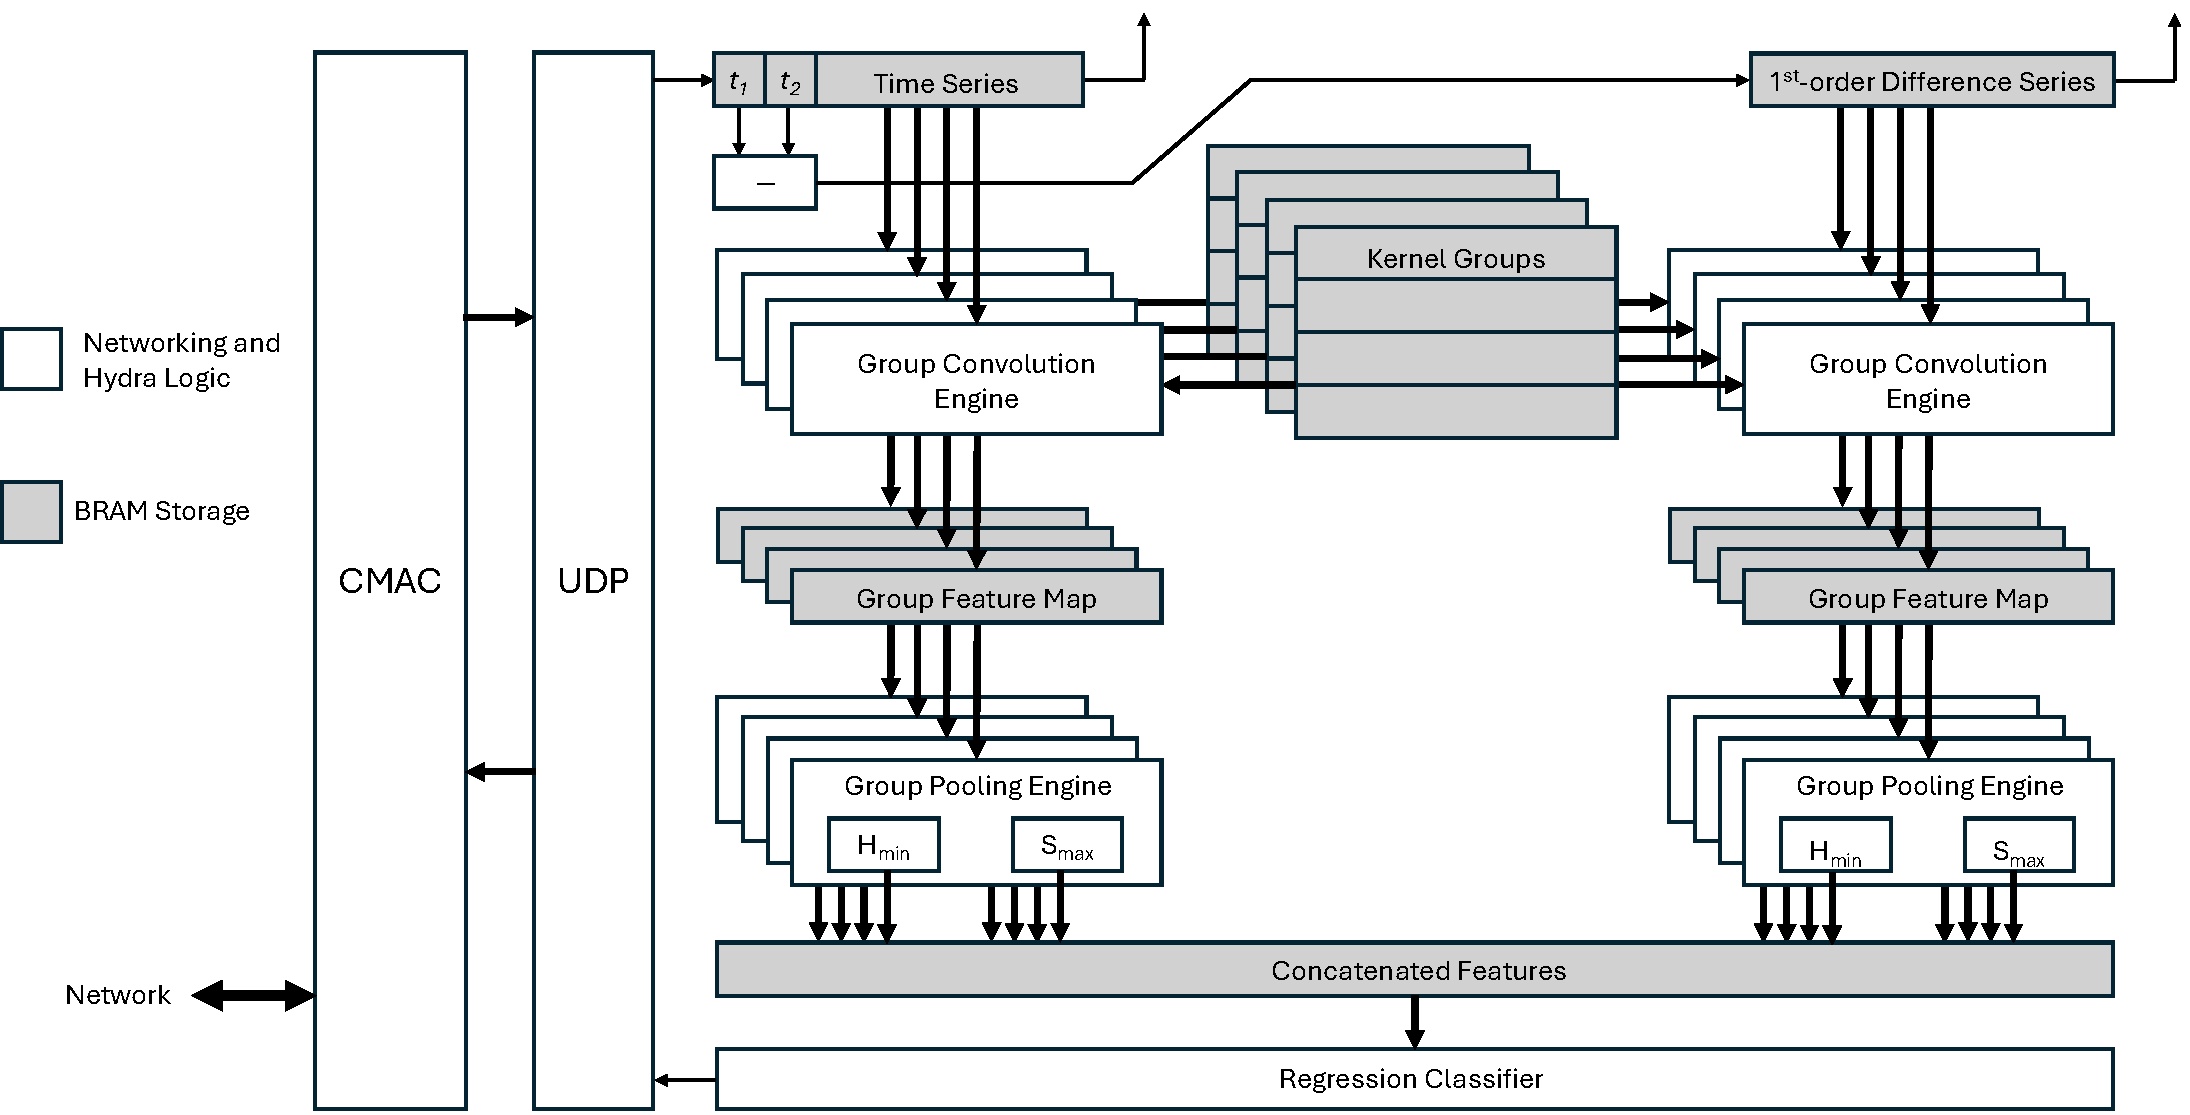
\includegraphics[width=1\linewidth]{Figures/Hydra_Arch.pdf}
\caption{FPGA accelerator for Hydra.}
\label{fig:Hydra_arch}
\end{figure*}


%\section{Convlution Engine Design}
%\label{sec:convolution_engine}

\begin{figure}[tp]
    \centering
        \begin{subfigure}{\linewidth}
      \centering
      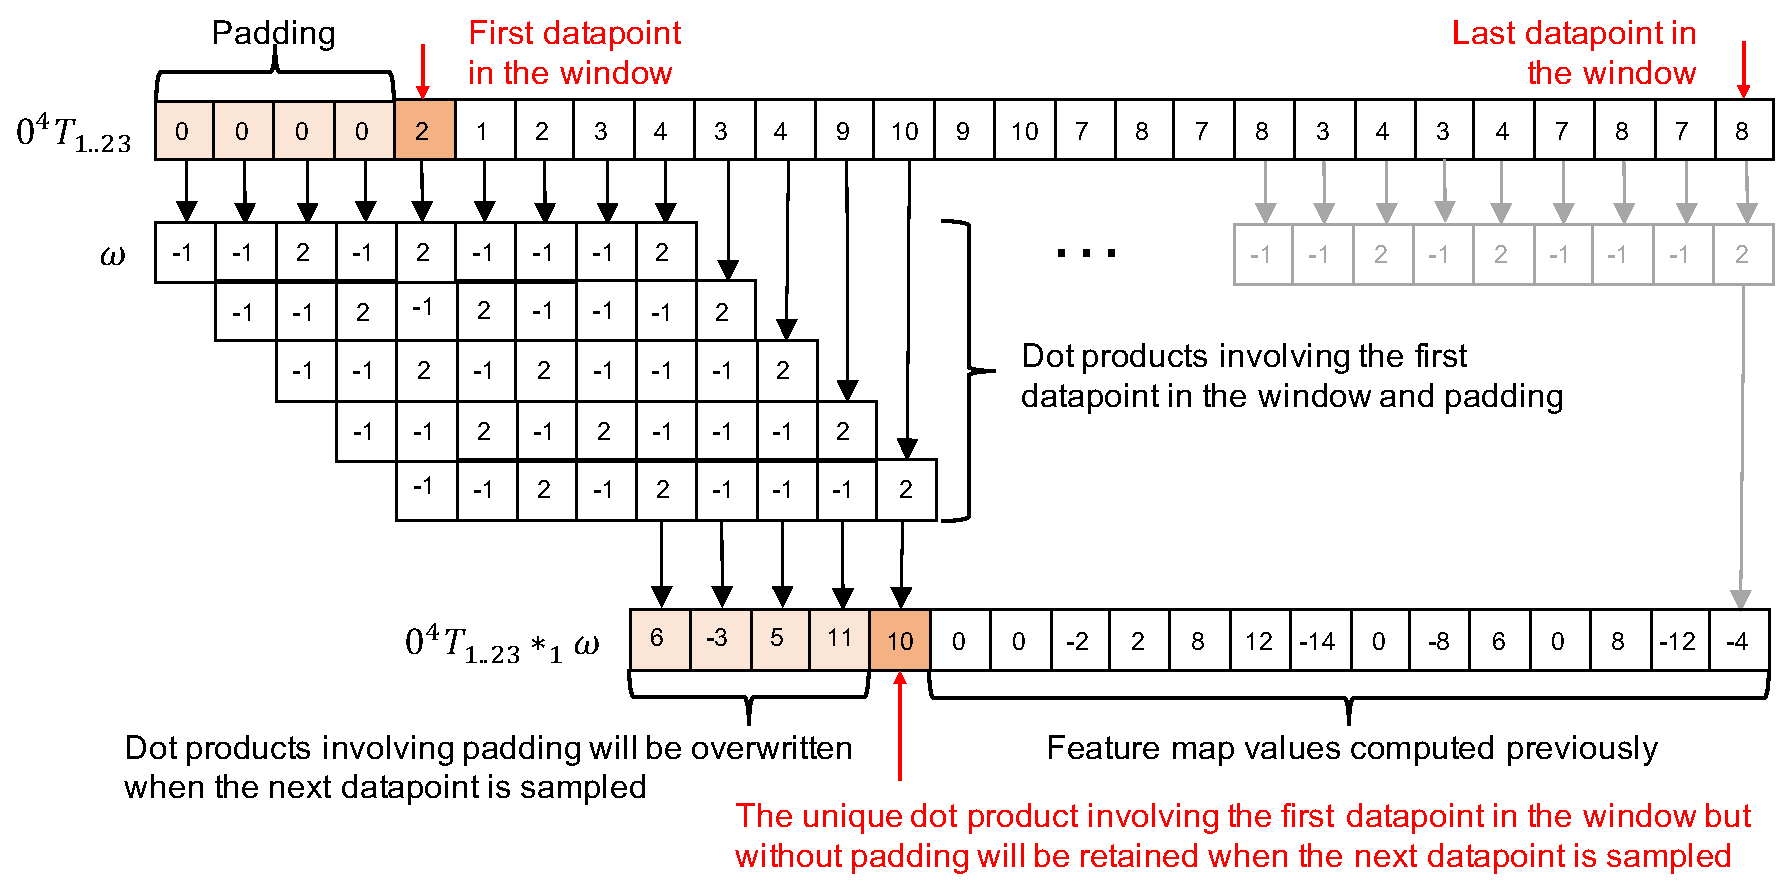
\includegraphics[width=\linewidth]{Figures/Convolution Engine-a.pdf}
      %\caption{}Convolution $0^4T_{1..n} *_1 \omega$}
      \label{fig:conv_eng_1}
    \end{subfigure}
    \begin{subfigure}{\linewidth}
        \centering
          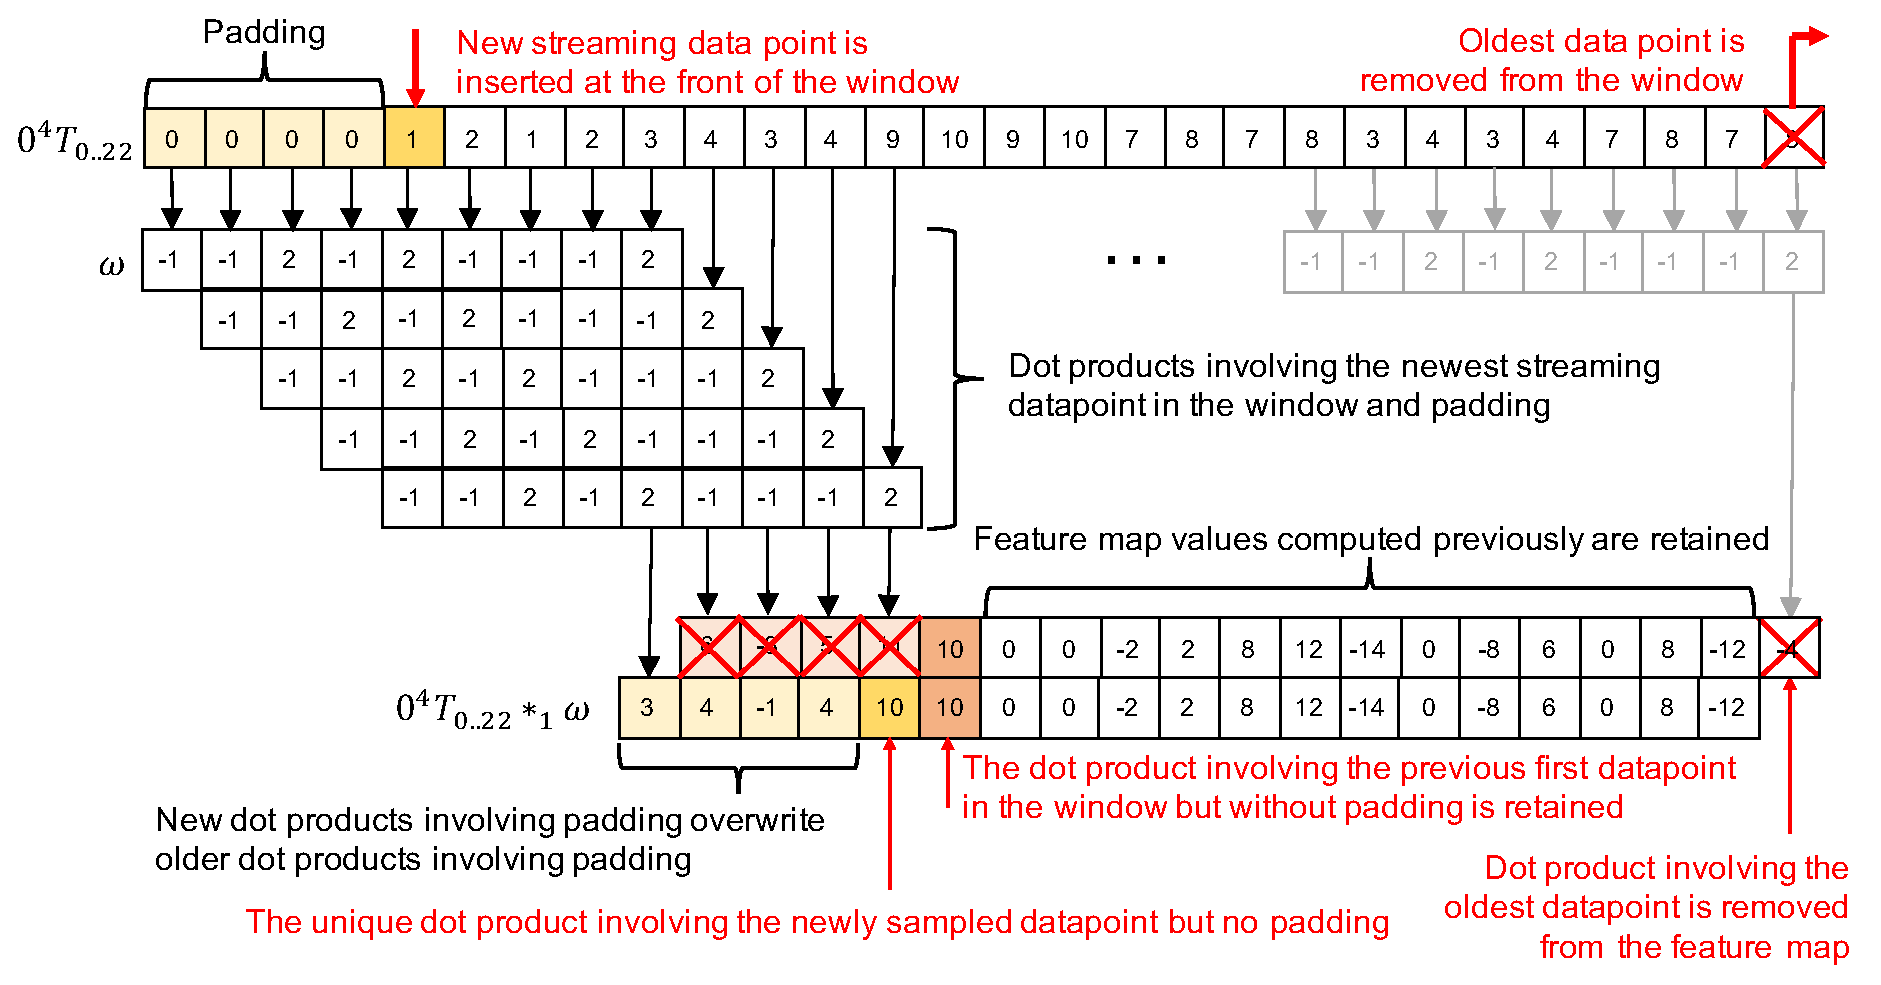
\includegraphics[width=\linewidth]{Figures/Convolution Engine-b.pdf}
        %\caption{}%Convolution $0^4T_{0..n-1} *_1 \omega$
        \label{fig:conv_eng_2}
    \end{subfigure}
    \caption{Dot product reuse when computing a convolution involving a padded time series before (top) and after (bottom) a new datapoint is added to the window.}
    \label{fig:convolution_engine}
\end{figure}

%\section{Arithmetic Operator Design}
%\label{sec:Arithmetic}

\subsection{MiniRocket/MultiRocket Floating-point Multiplication}
\label{sec:fp_mult}

All of the aforementioned classifiers are specified using 32-bit floating-point numbers and operators. 
%Recall that each convolutional kernel $\omega$ consists of nine scalar values, six of which are $-1$ and three of which are $2$. MiniRocket decomposes its kernel into two sub-kernels, $\langle-\textbf{1}\rangle$ (a vector containing nine scalar values of $-1$) and $\omega'$ containing six values which are zero and three which are $3$, such that $\omega = \langle-\textbf{1}\rangle + \omega'$. For example, $[-1, -1, 2, -1, 2, -1, -1, -1, 2] = \langle-\textbf{1}\rangle + [0, 0, 3, 0, 3, 0, 0, 0, 3]$. MiniRocket computes each convolution as $T * \omega = T*\langle-\textbf{1}\rangle + T*\omega'$. Our implementation eschews this decomposition for reasons described in the following subsections. 
%Let $T_{i,9}^d$ be a subsequence of time series $T$ starting at element $t_i$ and containing $9$ elements with dilation $d$, i.e., $T_{i,9}^d = \langle t_i, t_{i+(d-1)}, \ldots, t_{i+8(d-1)} \rangle$. MiniRocket computes its convolution
%MiniRocket is written using 32-bit floating-point numbers and operators; while it is certainly possible to explore training and inference for MiniRocket using reduced-precision floating-point and/or fixed point numeric formats, we leave such an exploration open for future work. 
A floating-point number is a tuple $\langle s, e, f \rangle$, where $s$ is a \textbf{sign bit}, $e$ is an \textbf{exponent} and $f$ is the \textbf{fractional} component, or \textbf{mantissa}; a floating-point value is computed as $(-1)^s\cdot2^{e-b}\cdot1.f$, where $b$ is a constant-valued bias term, and $1.f$ represents a fractional value in the range $[1, 2)$; special encodings are provided for $\pm 0$, $\pm \infty$, and not-a-number ($NaN$). A 32-bit \textbf{float} has $8$ exponent bits and $23$ mantissa bits. 

In MiniRocket and MultiRocket, each kernel $\omega$ consists of nine scalar values, six of which are $-1$ and three of which are $2$. 
Multiplication by $-1$ can be implemented by inverting the sign bit $s$ and multiplication by $2$ can be implemented by setting the bias term $b=0$ and incrementing $e$, with appropriate control logic for the case when $e$ overflows. %Multiplication by $3$, the constant favored in MiniRocket's software implementation, is somewhat more entailed; we omit details to conserve space. 
We propose a binary encoding for MiniRocket and MultiRocket kernels: $\{0 \rightarrow -1, 1 \rightarrow 2\}$; this enables a compact floating-point multiplier design for encoded constants $-1$ and $2$. 

Consider floating-point operation $X \times Y$, where $X$ is any value, and $Y$ is either $-1$ or $2$; we use lower-case $y$ to represent the binary encoding of $Y$. Our proposed floating-point multiplier is specified as:
\begin{equation}
    \langle XNOR(X.s, y), X.e + y, X.f\rangle.
\end{equation}
Convolution operators can compute dot products using the specialized floating-point multiplier, but must perform accumulation using standard floating-point operators. 

In our experiments, we never observed an instance where multiplying by $2$ caused the exponent to overflow, so we omit overflow handling logic as well as $\pm \infty$ and $NaN$. 
%A comparable multiplier for binary-encoded floating-point values of $-1$ and $3$ would involve non-trivial adjustments to both the exponent and mantissa. 

